%% ANEXOS
\hypertarget{estilo:anexo}{}

\chapter{ANEXO B - CICLO DE ASSIMILAÇÃO DE DADOS (CAD)}
\label{anexoB}

Convencionalmente, no Ciclo de AD (CAD) as informações são extraídas das observações - comumente esparsas, para reconstruir e/ou ajustar a estrutura das variáveis que representam os sistemas atmosféricos. Esta técnica combina o estado da atmosfera anteriormente predita por uma previsão de curto prazo (\textit{first guess}), normalmente de 6 horas, com dados observacionais recentes para produzir um estado atmosférico estimado e atualizado (a análise) e que é utilizada como condição inicial nos modelos de PNT, a partir do qual se gera uma nova previsão, \cite{kalnay03}. A este processo dá-se o nome de Ciclo de Assimilação de Dados (CAD) (esquematizado na \autoref{fig90}).

\begin{figure}[!hbp]
\centering
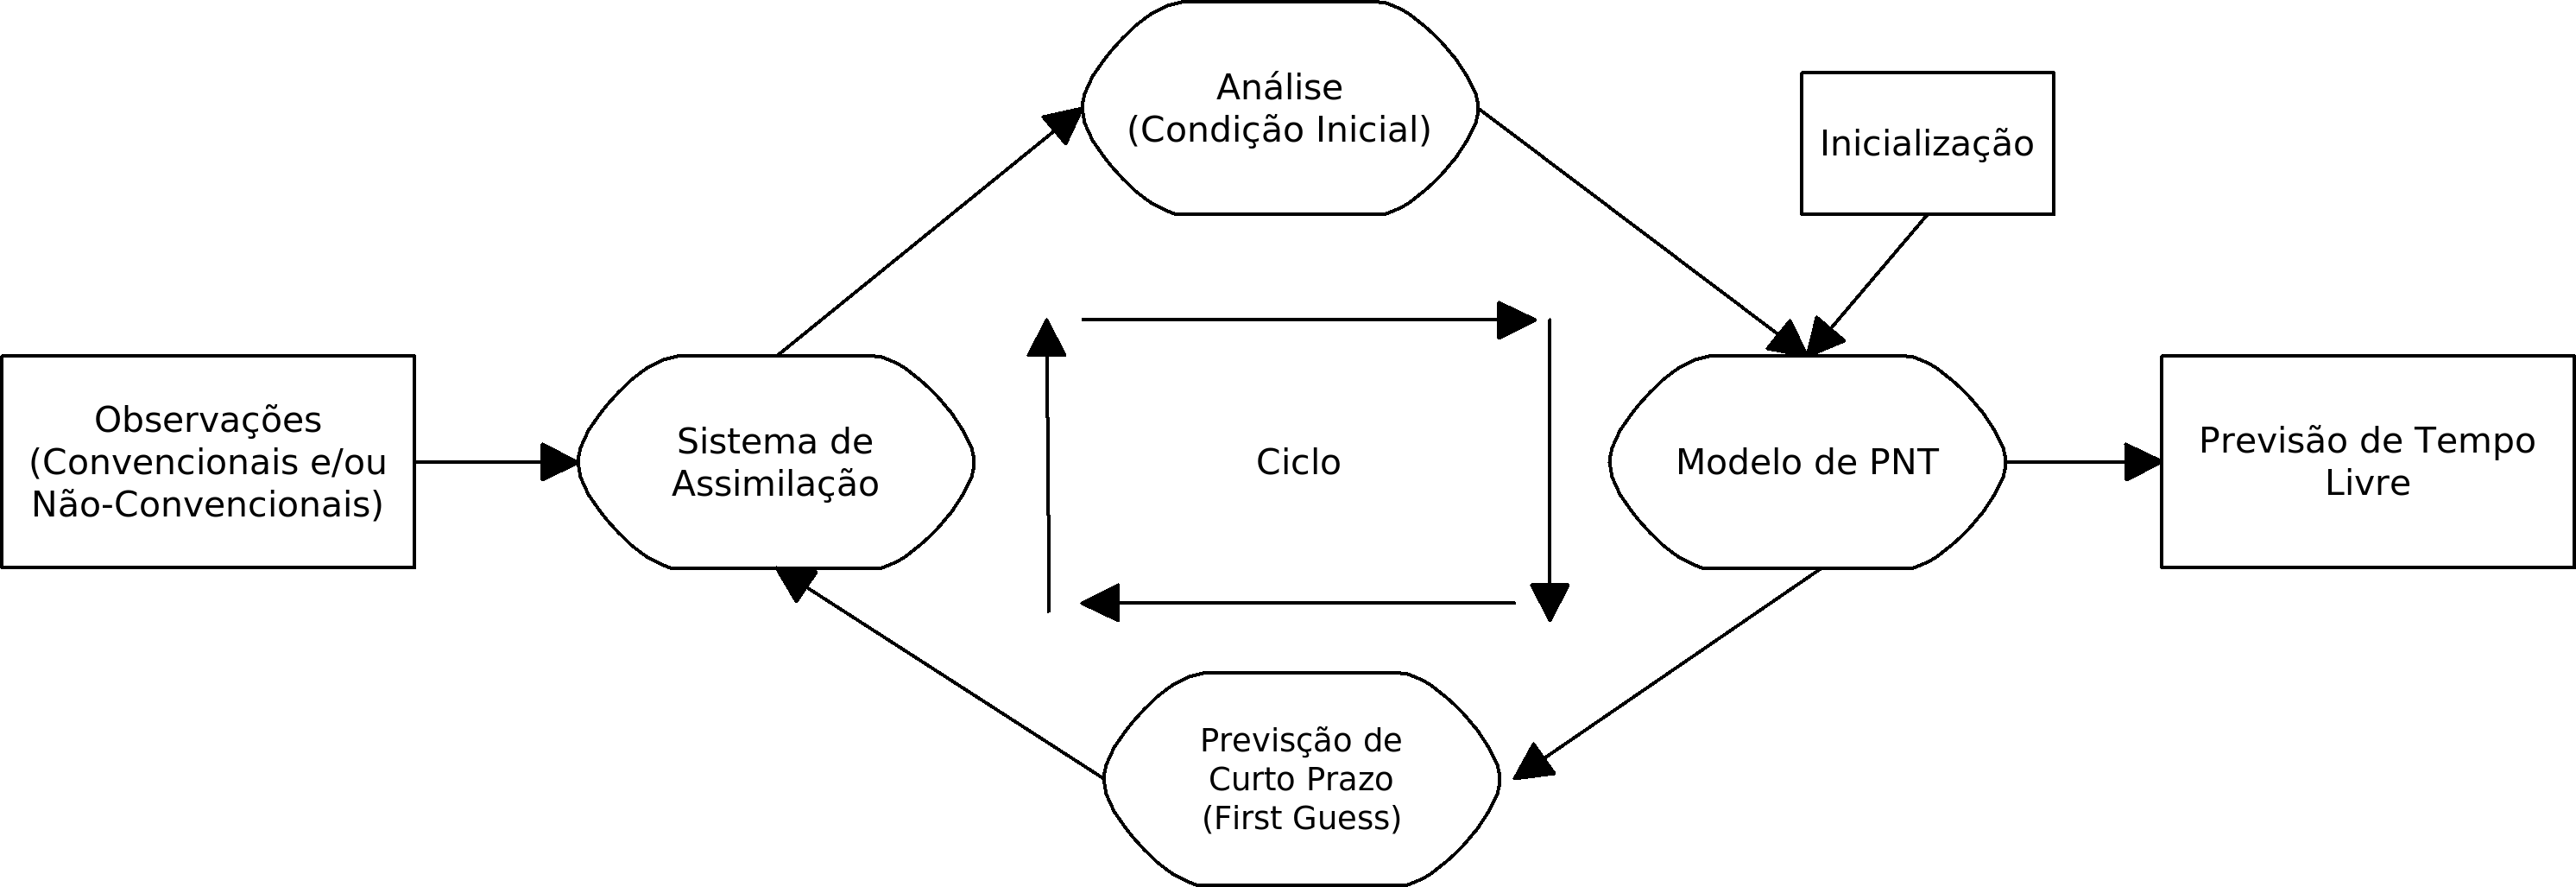
\includegraphics[height=4.5cm]{./figs/ciclo_ad.png}
\caption{Diagrama esquemático do Ciclo de Assimilação Contínuo.}
\label{fig90}
\end{figure}

Em etapas, o CAD pode ser dividido em quatro partes:

\begin{enumerate}
\item \textbf{Controle de Qualidade:} no início do CAD, são verificados os dados observados em termos da consistência da distribuição espaço-temporal. Os dados são comparados com os seus vizinhos e são verificados erros de codificação dos dados e de localização dos instrumentos de medição. Nesta etapa os dados podem ser rejeitados ou não;
\item \textbf{Análise Objetiva:} nesta etapa os dados observados são interpolados na grade do modelo e são feitas pequenas correções nos campos previstos do \textit{first guess}. Nesta etapa o \textit{first guess} é preparado para geração da análise, que pode ser feita através de métodos diversos: Interpolação Ótima (IO em 3 ou 4 dimensões), Variacional ou filtro de Kalman (3DVar ou 4DVar). No CPTEC, por exemplo, é utilizado o \textit{Physical-space Statistical Analysis System} (PSAS) que é um esquema híbrido com características de IO e 3DVar \cite{courtieretal98};
\item \textbf{Inicialização:} a partir da análise, as condições iniciais de integração devem ser livres de oscilações ou ondas espúrias (e.g. ondas de gravidade inercial). Há vários métodos de inicialização: Modos Normais Linear e Não Linear (MNL e MNNL), Filtro Digital (FD), Euler-\textit{Backward} (esquema de Matsuno) e outros. Normalmente estes esquemas são realizados pelo modelo de previsão. Também, observa-se que quando a análise é produzida por métodos variacionais não é necessária a utilização de inicialização. No sistema Eta+RPSAS, esta fase é realizada utilizando um FD, o qual é responsável pelo processo de inicialização dos dados inseridos no modelo após a geração da análise;
\item \textbf{Previsão (de curto prazo e livre):} nesta etapa é gerado o \textit{first guess} do próximo ciclo de análise/previsão, que normalmente é uma previsão de 3 ou 6 horas (nos modelos regional e/ou global, respectivamente). Nesta etapa utiliza-se o modelo de PNT, o qual inclui as parametrizações físicas necessárias para assegurar que se não for atualizado com novas observações, o estado (previsão) por ele gerado será próximo do verdadeiro. Isto garante também que na falta de dados o \textit{first guess} produzido pelo sistema de assimilação/previsão permaneça plausível. A partir do \textit{first guess}, é gerada a análise que é utilizada como condição inicial do modelo PNT que é utilizado para previsões livres de até 3 ou 4 dias para modelos regionais e de até 7 dias para modelos globais.
\end{enumerate}
